\section{Read/Write Images}
\label{sec:warmup1}
    \subsection{Problem}
        In this exercise, we were provided with two datasets. The objective was to proficiently load the data using PyTorch's dataloaders and dataset APIs, and subsequently, successfully generate matplotlib plots by writing the images.
    \subsection{Solution}
        
    To load the provided dataset, custom PyTorch dataset classes were crafted. These classes offer flexibility to handle datasets of various types and formats. The torchvision.io.read\_image function is employed for reading PNG/JPG images, while the pydicom library is utilized for reading DICOM data.
    
    \subsubsection*{Transformations}
        \begin{figure}[b]
            \begin{subfigure}[t]{\linewidth}
                \centering
                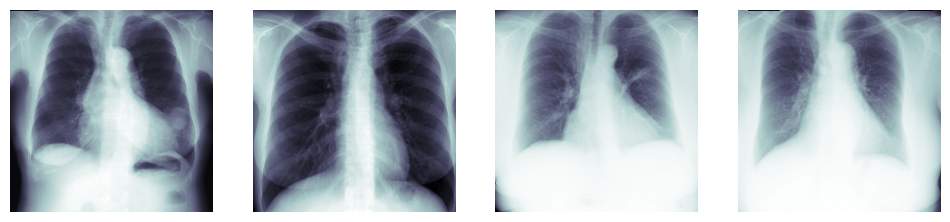
\includegraphics[width=\linewidth]{images/chest-xray-output.png}
                \caption{PNG/JPG dataset}
                \label{fig:png-image}    
            \end{subfigure}
            \begin{subfigure}[t]{\linewidth}
                \centering
                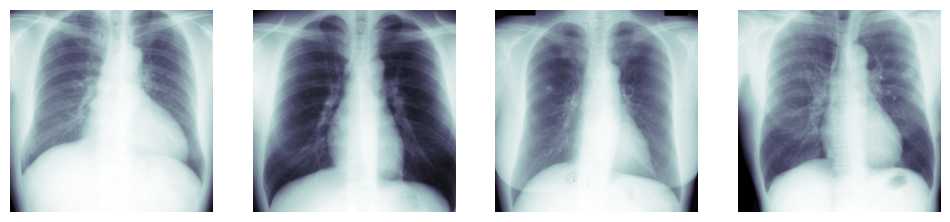
\includegraphics[width=\linewidth]{images/dicom.png}
                \caption{DICOM dataset}
                \label{fig:dicom-image}
            \end{subfigure}
            \caption{XRay images batch}
            \label{fig:xray-images}
        \end{figure}
        \begin{itemize}
            \item When PNG/JPG images were loaded, a resize transformation was applied to change the images to a size of $256$x$256$. \Cref{fig:png-image} displays a batch of 4 images from the PNG/JPG dataset.
            \item After loading DICOM data, a sequence of transformations was employed. At first, the image type is converted from uint16 to uint8, because PyTorch resize function does not support uint16 dtype. Subsequently, the tensor is converted to a PIL image, and the image is resized. Following the dataset loading, all the images are plotted in a matplotlib plot. \Cref{fig:dicom-image} displays a batch of 4 images from the DICOM dataset.
        \end{itemize}
    